%gibt an: Papierformat, Schriftgr��e
\documentclass[a4paper,german,12pt]{article}
\setlength{\parskip}{0.2cm}
\setlength{\parindent}{0cm}
%-----------------------------------------------------------------------------------------------------------------------------
%�bersetzung von E in D
\usepackage{ngerman}
%Einstellung der Randabst�nde
\usepackage[lmargin={2.5cm},rmargin={2.5cm},tmargin={1.5cm},bmargin={2.5cm}]{geometry}
%zur Einbindung von Graphiken
\usepackage{graphicx}
%Bearbeitung von Kopf- und Fusszeile
\usepackage{fancyhdr}
%Schriftart
\usepackage{helvet}
%stellt unabh�ngige Textmarken zu Verf�gung
\usepackage{extramarks}
%aktiviert eine Umgebung in der der Mathematikmodus aktiv ist
\usepackage{amsmath}
%aktiviert eine Umgebung in der der Mathematikmodus aktiv ist
\usepackage{amsthm}
%aktiviert eine Umgebung in der der Mathematikmodus aktiv ist
\usepackage{amssymb}
%aktiviert Hyperlinks
\usepackage{hyperref} 
%Stellt das Eurozeichen � zu Verf�gung
\usepackage[right]{eurosym}
%�bersetzt die Tastatureingaben f�r LaTex
%\usepackage[latin1]{inputenc}
\usepackage{fancybox}
\usepackage{xcolor}
\usepackage{color}
\usepackage{float}
\usepackage{framed}
\usepackage{url}
\usepackage[ansinew]{inputenc}

%\usepackage[square]{natbib}

%Weitere
\usepackage{bibgerm} %Bibliothek

\usepackage{booktabs}
\usepackage{tabularx} %Tabellen, die sich der Seitenbreite anpassen

\usepackage{multirow} % Verbundene Zellen in Tabellen

\usepackage{rotating} % Quergestellte Tabellen
\usepackage{rotfloat}

\usepackage[bottom]{footmisc} %Fu�noten immer am Ende der Seite

%\usepackage[T1]{fontenc}
\usepackage[final]{microtype}

%Definitionen

\newtheoremstyle{mystyle}% name
{10pt}% Space above
{10pt}% Space below
{\itshape}% Body font
{}% Indent amount: 
{\bfseries}% Theorem head font
{:}% Punctuation after theorem head
{0.5em}% Space after theorem head
{\thmname{#1}\thmnumber{ #2}:\thmnote{ #3}}% Theorem head 

\theoremstyle{mystyle}% default
\newtheorem{definition}{Definition}
\numberwithin{equation}{section}
\renewcommand{\proofname}{Beweis}

%Paragraphen

\newcommand{\myparagraph}[1]{\paragraph{}\mbox{}\\}


%-----------------------------------------------------------------------------------------------------------------------------------------
\renewcommand{\baselinestretch}{1.2}
\fancyhead[LO]{\slshape \small \firstleftmark}
\fancyhead[RO]{\normalsize\thepage} \fancyfoot{}
\begin{document}
%-----------------------------------------------------------------------------------------------------------------------------------------
%Titelseite

\begin{titlepage}
% font / Schriftart
%------------------	
\begin{figure}[htbp]
  %\centering
  \begin{minipage}[t]{0.4\textwidth} 
    
\includegraphics[scale=0.75]{0_Logos/kit.jpg}  
    
  \end{minipage}
  \hfill
  \begin{minipage}[b]{0.3\textwidth} 
	\begin{flushleft}
		
\includegraphics[scale=0.09]{0_Logos/aifb.png}     
	\end{flushleft}
	\begin{flushleft}
		\tiny\textbf{Institut f�r Angewandte Informatik}
		\textbf{und Formale Beschreibungsverfahren}
	\end{flushleft}
  \end{minipage}
\end{figure}

\vspace*{1.5cm}
\leftskip=4cm
		\textbf{{\Huge %TODO
		Titel der Abschlussarbeit}\\
		%{\Huge
		%[auch mehrzeilig m�glich]}
		}
		\vspace*{1.5cm}\\
		{\Large Bachelorarbeit}\\
		{\Large von} \\
		{\Large Marius Wodtke}
		\vspace*{3.5cm}\\
		an der Fakult�t f�r Informatik
		\vspace*{0.5cm}\\
		In dem Studiengang\\
		Informatik (B.Sc.)
		\vspace*{1.5cm}\\
		eingereicht am 01.01.01 %TODO Datum
		beim\\
		Institut f�r Angewandte Informatik\\
		und Formale Beschreibungsverfahren\\
		des Karlsruher Instituts f�r Technologie
		\vspace*{2.5cm}\\
		Referent: Prof. Dr. Hartmut Schmeck
		\\
		Betreuer: Kaibin Bao
		\vspace*{1.5cm}\\
		{\footnotesize KIT -- Universit�t des Landes Baden-W�rttemberg und}\\
		{\footnotesize nationales Forschungszentrum in der Helmholtz-Gemeinschaft}\\
		\hfill

\end{titlepage}


\thispagestyle{empty}\cleardoublepage

\mbox{}\thispagestyle{empty}
\cleardoublepage

\mbox{}\thispagestyle{empty}

\vspace*{1cm}

{\Large \textbf{Eidesstattliche Erkl�rung}} 

\bigskip

Ich versichere hiermit wahrheitsgem��, die Arbeit und alle Teile daraus selbst�ndig angefertigt, alle benutzten Hilfsmittel vollst�ndig und genau angegeben und alles kenntlich gemacht zu haben, was aus Arbeiten anderer unver�ndert oder mit Ab�nderung entnommen wurde.\\

\vspace{1cm}
 
\textit{Karlsruhe, den DATUM} \hspace{4cm} \textit{NAME} \\

\thispagestyle{empty}\cleardoublepage

\mbox{}\thispagestyle{empty}
\cleardoublepage
\rmfamily \pagestyle{fancy} \setcounter{secnumdepth}{4}


\pagenumbering{roman}
\setcounter{page}{3} 
\tableofcontents
\newcounter{roemisch} 
\setcounter{roemisch}{\value{page}}
\markboth{ABK�RZUNGSVERZEICHNIS}{Abk�rzungsverzeichnis}
\section*{Abk�rzungsverzeichnis}
\begin{table}[h]
    \begin{tabular}{rl}
    NILM & Non-intrusive load monitoring\\
    KNN & K�nstliches Neuronale Netz\\
    ESHL & Energy Smart Home Lab\\
    MLP & Multi Layer Perceptron\\
    \end{tabular}%
\end{table}%

\cleardoublepage
\listoffigures
\cleardoublepage
\listoftables
\cleardoublepage

\setcounter{page}{2} \pagenumbering{arabic}

\interfootnotelinepenalty=10000 % Keine Seitenumbr�che bei Fu�noten

 % % % % % % % % % % % % %INHALTE % % % % % % % % % % % % % %
 \section{Einleitung}
\label{Einleitung}

%\subsection{Motivation}
%\label{Motivation}
	Energie zu sparen ist seit Langem ein Ziel der Umweltpolitik, dennoch steigt der Energieverbrauch in Industriel"andern kontinuierlich und es werden nach wie vor Wege gesucht, diesen zu senken. 
	In den USA verursachen private Haushalte 40\% des CO2-Aussto{\ss}es \cite{vandenbergh2008individual} und stehen deshalb im Fokus vieler Programme zum Energiesparen. \\
	Je nach Studie besteht f"ur die Haushalte ein Einsparungspotential von bis zu 20\% \cite{armel2013disaggregation} f"ur dessen Energieverbrauch, Fischer \cite{fischer2008feedback} untersucht mehrere dieser Studien und beschreibt ein durchschnittliches Einsparungspotential von 5-12\%. 
	Um dieses Einsparungspotential auszunutzen, muss der Nutzer regelm"a{\ss}ig und m"oglichst genau "uber seinen Verbrauch aufgekl"art werden. 	%TODO Graphik Armel
	\begin{figure}[ht]
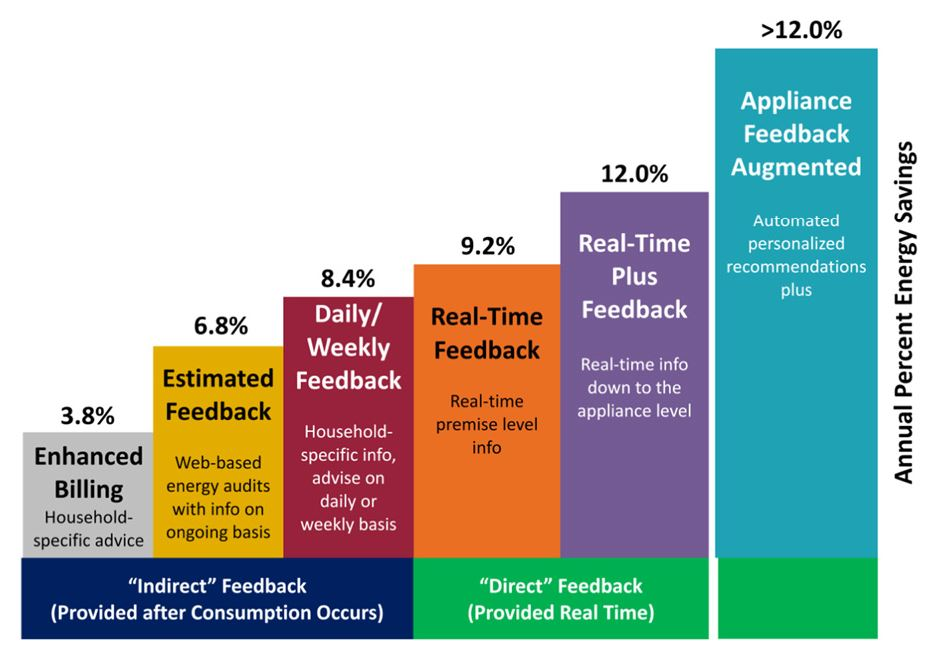
\includegraphics[width=\textwidth]{1_Grafiken/fig1armel.jpg}
	\caption[Einsparungpotentiale nach Ma{\ss}nahme]{Grafik zu Einsparpotetialen je nach getroffener Aufkl"arungsma{\ss}nahme aus \cite{armel2013disaggregation}}
\label{potentiale}
\end{figure}

	Er kann sich oft nicht mit seinem Verbrauch identifizieren, weil dieser intransparent und durch die langen Rechnungsintervalle nicht pr"asent ist. \\
	Damit der Nutzer anf"angt sich selbst zu kontrollieren, muss er begreifen, dass sich sein Verhalten auf seinen Verbrauch auswirkt und er ihn auch durch die gezielte Ver"anderungen seines Handelns senken kann \cite{fischer2008feedback}.\\
	Non-intrusive load monitoring (NILM) bietet nun die Chance dem Nutzer eine regelm"a{\ss}ige, detaillierte R"uckmeldung zu seinem Energiekonsum zu geben, Kolter und Matthew \cite{kolter2011redd} beschreibt NILM als die Aufgabe aus einem, f"ur den gesamten Haushalt messenden Stromz"ahler, R"uckschl"usse "uber die elektrische Last einzelner Ger"ate zu ziehen.
	Ein solches System wird dem Konsumenten helfen, verschwenderische Verhaltensweisen und Ger"ate zu identifizieren ohne den Haushalt mit vielen digitalen Z"ahlern f"ur die individuellen Ger"ate ausr"usten zu m"ussen, wie es derzeit z.B. mit sogenannten \textit{Energiekostenmessger"aten} auf Steckerbasis praktiziert wird.

\subsection{Fragestellung}
\label{Fragestellung}
 	Viele Systeme zur Disagregation oder zu verschiedenen Vorhersage-Aufgaben benutzen Ans"atze des Maschinellen Lernens. Sie ben"otigen annotierte (gelabelte) Trainingsdaten, um robuste Modelle zu erzeugen. Annotieren bedeutet in diesem Zusammenhang, die Daten mit Metadaten wie etwa dem Ger"atezustand zu versehen. Mehr Trainingsdaten f"uhren in der Regel zu besseren Modellen, die Annotation ist allerdings sehr aufw"andig, weil sie manuell erfolgen muss. Der Ansatzpunkt dieser Arbeit ist, das Problem der Disagregation auf ein Ger"at zu reduzieren und so zu vereinfachen. Nun kann man ein robustes Modell mit nur wenigen Trainingsdaten erstellen und mit diesem dann eine gro{\ss}e Menge an Daten schnell annotieren. Diese gelabelten Daten sollen dann wiederum als Trainingsdaten f"ur schwierigere Aufgaben verwendet werden. 
	Aufgabe dieser Bachelorarbeit ist es ein System zu entwickeln, welches in der Lage ist die Zust"ande von ausgew"ahlten Ger"aten in einem disaggregierten Lastgang zu klassifizieren und so eine Segmentierung f"ur diese Ger"ate zu erstellen. Dies beinhaltet sowohl die n"otige Vorverarbeitung der Daten sowie eventuelle nachtr"agliche Formatierungen. Die eigentliche Klassifikation soll mit K"unstlichen Neuronalen Netzen (KNN) stattfinden, dabei sollte eine m"oglichst hohe Akkurarit"at erreicht werden, da Systeme, die mit den resultierenden Daten trainiert werden keine M"oglichkeit haben Fehler, die bereits in den Trainingsdaten sind, zu korrigieren. 
Au{\ss}erdem soll versucht werden aus den klassifizierten Daten wieder einen Lastgang zu erstellen. Dies soll die M"achtigkeit der Segmentierung der Ger"atezust"ande untersuchen und feststellen ob man zuverl"assig den Lastgang des Ger"ats vorhersagen kann, wenn es seine Zustandsfolge im Voraus bekannt gibt. 

\subsection{Weiterer Aufbau}
\label{Weiterer Aufbau}
	Im folgenden Kapitel~\ref{Datensatz} werden die verwendeten, disaggregierten Energiedatens"atze beschrieben. Insbesondere werden die gemessenen Werte und die daraus berechenbaren Werte untersucht. 
	Kapitel~\ref{Vorverarbeitung} gibt zun"achst einen "Uberblick "uber die aktuelle Forschung im Bereich Vorverarbeitung der Daten und Feature-Auswahl, anschlie{\ss}end werden die f"ur diese Arbeit verwendeten Vorverarbeitungsschritte und Features erl"autert.
	In Kapitel~\ref{Klassifizierung} soll schlie{\ss}lich die eigentliche Klassifizierung beschrieben werden, hier werden insbesondere das verwendete Netz und die Trainingsmethoden besprochen. Auch hier wird es einen kurzen "Uberblick "uber die aktuelle Forschung geben.
	In Kapitel~\ref{Generierung} wird die Generierung eines Lastprofils aus dem Zustandsprofil erl"autert. Es wird ein Ansatz aus der aktuellen Forschung beschrieben und auf dieses Problem adaptiert. 
	In Kapitel~\ref{Evaluation} findet die Evaluation statt, hier werden verschiedene Klassifikationsaufgaben ausgef"uhrt und ausgewertet. 
	Am Schluss steht das Fazit in Kapitel~\ref{fazit}, in dem die Ergebnisse zusammengefasst und mit urspr"ungliche Fragestellung verglichen werden. 
 
 \section{Datensatz}
\label{Datensatz}

Die verwendeten Daten stammen aus dem \textit{KIT Smart Home Lab}. Sie wurden "uber fast 3 Jahre zwischen dem 22.08.2011 und dem 31.07.2014 aufgezeichnet, weisen aber einige L"ucken auf. F"ur die Messungen wurden mehrere Smart Meter verwendet, bei Gro{\ss}verbrauchern wie etwa dem Boiler wurden dabei alle drei Phasen gemessen, sie sind durch die Nummer des Smart Meters in den Daten identifizierbar. Bei den restlichen Ger"aten wurde nur je eine Phase gemessen, das hei{\ss}t, dass je 3 Ger"ate an einem Smart Meter angeschlossen sind, sie sind durch die Nummer des Smart Meters in Kombination mit Nummer des verwendeten Ports identifizierbar. Wie viele Phasen zur Messung eines Ger"ats verwendet wurden l"asst sich dem Controller entnehmen.
\begin{table}[h]
\begin{tabular}{l|l|l|l|l|l}
UUID & Name & Klassifikation & Controller & Meter & Port \\
\hline
...-5602c0a80114 & DRYER & APPLIANCE & 1 & 3 & 0 \\
...-5604c0a80114 & WASHINGMACHINE & APPLIANCE & 1 & 7 & 2
\end{tabular}
\end{table}



\subsection{Gemessene Daten}
\label{Gemessene Daten}

Die Daten des \textit{KIT Smart Home Lab} besitzen folgendes Format. \\
\begin{table}[h]
\begin{tabular}{l|l|p{1cm}|p{1cm}|p{1cm}|p{1cm}|p{1cm}|p{1.2cm}|p{2cm}}
Unixtime & UUID & Con-troller & Meter & Port & Span-nung & Strom-st"arke & Wirk-leistung & Wirkl. \newline aggregiert \\
\hline
1382291846 & ...-5604c0a80114 & 1 & 7 & 2 & 218.5 & 8.96 & 1956 & 145550  \\
1315269463 & ...-5602c0a80114 & 1 & 3 & 0 & 223.8 & 13.16 & 2950 & 38300 \\
1315269465 & ...-5602c0a80114 & 1 & 3 & 0 & 223.9 & 12.5 & 2796 & 38300
\end{tabular}
\end{table}

Controller, Meter und Port werden, wie oben beschrieben, verwendet, um einen Datenpunkt einen eindeutigen Ger"at zuzuordnen. Hier ist zu beachten, sich diese Werte immer nur gemeinsam verwendet werden d"urfen.
Die Spalte mit der UUID-Zuordnung wird ignoriert, denn sie enth"alt ebenfalls die Information um welches Ger"at es sich handelt und ist somit Redundant zu Controller, Meter und Port. \\
Ein Datenpunkt enth"alt die gemessene Spannung, die Stromst"arke und die Wirkleistung. Es wird zus"atzlich die aggregierte Wirkleistung gemessen, welche aber zun"achst ignoriert wird, da sie sich aus der Wirkleistung berechnen l"asst. \\
Eine Besonderheit stellt das Aufzeichnungsintervall dar. Die Smart Meter erzeugen jede Sekunde einen neuen Datenpunkt f"ur jeden Port, dieser wird aber nur gespeichert, wenn sich die Wirkleistung im Vergleich zum letzten gespeicherten Punkt um 5 Watt Wirkleistung unterscheidet. So werden insbesondere lange \textit{Off} Phasen auf einen Datenpunkt komprimiert, es gehen aber auch kleinere Schwankungen in der Wirkleistung von sehr verbrauchsarmen Ger"aten verloren.


\subsection{Berechnete Daten}
\label{Berechnete Daten}

Die Messung von Spannung und Stromst"arke erlaubt es eine Vielzahl von Energiewerten zu berechnen, in diesem Abschnitt werden die Schein- und Blindleistung vorgestellt, das Kapitel zur Vorverarbeitung wird zus"atzlich eine Form der Normalisierung vorstellen. 
Die Scheinleistung ist das Produkt aus Spannung und Stromst"arke und ist die gesamte, aus dem Netz gezogene Leistung:\\ $Scheinleistung = Spannung * Stromst"arke$\\[0.5cm]
Zur Berechnung der Blindleistung werden Schein- und Wirkleistung genutzt, die Blindleistung ist dabei Leistung, die aus dem Netz gezogen wird ohne tats"achlich genutzt zu werden:\\ $Blindleistung = \sqrt{Scheinleistung^2 - Wirkleistung^2}$ \\


\subsection{Die Waschmaschine}
\label{Die Waschmaschine}

Die Waschmaschine ist ein besonders interessantes Ger"at f"ur die Klassifikation, denn sie hat nicht nur einen \textit{On-} und einen \textit{Off-Zustand}, sondern einen Motor, der mit verschiedenen Drehzahlen laufen kann, ein Heizelement und eine Pumpe. F"ur die Waschmaschine existieren au{\ss}erdem einige annotierte Waschg"ange die als Trainingsdaten verwendet werden k"onnen.\\
\begin{table}[h]
\begin{tabular}{l|l|l|l|l}
Profil & Startzeit (Unix) & Endzeit (Unix) & Dauer (Sekunden) & Datum \\
\hline
Profil 0 & 1382290611 & 1382296244 & 5633 & 20.10.2013 \\
Profil 1 & 1382363246 & 1382369468 & 6222 & 21.10.2013 \\
Profil 4 & 1382900551 & 1382905960 & 5409 & 27.10.2013 \\
Profil 5 & 1383173215 & 1383180425 & 7210 & 30.10.2013 \\
Profil 8 & 1384066710 & 1384072260 & 5550 & 10.11.2013
\end{tabular}
\end{table}\\
Die Waschg"ange sind mit sechs verschiedenen Klassen Sigma 0 bis Sigma 5 annotiert, Sigma 0 ist der \textit{Off-Zustand}. Sigma 1 ist ein normaler Schleudervorgang, hier sind Phasen mit 200-350 Watt und dazwischen kurze Pausen mit ca. 4 Watt Verbrauch typisch.
Sigma 2 ist ein Heizvorgang, dieser kennzeichnet sich durch einen Verbrauch "uber 1700 Watt.
Sigma 3 und Sigma 4 sind Pumpvorg"ange und werden durch Verbrauchspitzen von wenigen Sekunden charakterisiert. Unterschieden werden sie anhand der H"ohe der Spitze, ein Vorgang Sigma 4 folgt immer auf einen Vorgang Sigma 3 mit einem Abstand von 50 bis 80 Sekunden.
Sigma 5 ist das Ausschleudern, es ist ebenfalls ein Schleudervorgang, der aber im Gegensatz zu Sigma 1 ohne Pausen ausgef"uhrt wird. (Bild Profil 0 mit Klassen angezeichnet)



 \section{Vorverarbeitung}
\label{Vorverarbeitung}
Verfahren des maschinellen Lernens sind Daten-getriebene Verfahren. Die Qualit"at des Ergebnisses der Klassifizierung ist also in besonderem Ma{\ss}e abh�ngig von der Qualit"at und Quantit"at der Daten. Die Vorverarbeitung soll durch m"ogliche Filterungen und Normalisierungen die Qualit"at des Datensatzes sichern und durch die Auswahl und Berechnung bestimmter Merkmale, den sogenannten Features, dem von dieser Arbeit verwendeten neuronalen Netz die Unterscheidung der verschiedenen Klassen m"oglichst einfach machen.\\
An der Klassifizierung beziehungsweise der Vorhersage von Energiedaten wird bereits seit "uber 20 Jahren geforscht und es wurden viele verschiedene Vorverarbeitungsschritte und aussagekr"aftige Features untersucht. Deshalb wird im Folgenden zun"achst eine "Ubersicht "uber die bisherige Forschung im Bereich der Vorverarbeitung gegeben und anschlie�end untersucht, welche Features f"ur die Unterscheidung verschiedener ger"ateinterner Zust"ande in Frage kommen.

\subsection{Stand der Technik}
\label{Stand der Technik}
	Die Wirkleistung ist das urspr"unglichste Merkmal um die Zust"ande von Ger"aten zu unterscheiden.
	Sie gibt die elektrische Leistung an, die von einem Ger"at in andere Leistungen (z.B. W"arme oder Bewegung) umgewandelt werden kann.  %TODO Verweis finden
	Oft wird die Wirkleistung durch gr"obere Quantisierung oder Normalisierung gegl"attet, um die Erkennung der Klassen zu vereinfachen. \cite{hart1992nonintrusive} verwendet hierzu folgende Formel:\\
	\begin{center}
	$P_{norm} (t) = (\frac{U_{nenn}}{U(t)})^2*P(t)$ \\ 
	mit Wirkleistung $P(t)$ und Spannung $U(t)$, die Nennspannung $U_{nenn}$ betr�gt in Europa 230 Volt.\\
	\end{center}
	Die Normalisierung bietet den Vorteil, dass sie nicht verlustbehaftet ist und wird deshalb h"aufig verwendet, wenn die Spannung gemessen wurde.\\
	Mit der Wirkleistung allein ist man jedoch nicht in der Lage Ger"ate mit sehr "ahnlichem Verbrauch zu unterscheiden, ein Beispiel w"aren hier ein 2kW Motor und ein 2kW Heizelement. 
	 Diese lassen sich mit Hilfe der Blindleistung, welche nicht in andere Leistungen umgewandelt wird, unterscheiden, weil der Motor als induktiver Verbraucher mehr Blindleistung als das Heizelement aus dem Stromnetz zieht. %TODO Grafik Hart und WaMa KIT
	 Nachteil hier ist jedoch, dass die Blindleistung (und auch die Spannung) zus�tzlich gemessen werden muss, dies kostet gegebenenfalls Geld \cite{zeifman2011nonintrusive}. \\
	 Vergleicht man jedoch eine 60W Gl"uhbirne und einen Laptop mit einem 60W Netzteil, dann stellt man fest, dass diese sich auch unter Hinzunahme der Blindleistung kaum unterscheiden lassen \cite{laughman2003power}. 
	 Hier hilft die Betrachtung von Micro Level Features. 
	 Dabei werden die Wellenformen und die harmonischen Komponenten des Frequenzspektrums verwendet, um Verbraucher zu unterscheiden. Laughman et al. \cite{laughman2003power} zeigen z.B., dass sich Gl�hbirne und Netzteil in der 3. harmonischen Komponente deutlich unterscheiden.
	 Zus"atzlich ver"andern viele Ger"ate die Wellenform des Stroms, so dass in diesem Bereich weiteres Potential f�r die Unterscheidung verschiedener Ger"ate vorliegt \cite{liang2010load}. \\ %TODO evtl Grafik Spektrum/Wellenform
	 Micro Level Features bieten sehr gute Unterscheidungsm"oglichkeiten, ben"otigen aber auch ein sehr hochfrequent aufgel"ostes Signal, "ublich sind mehrere kHz. Anderson et al. \cite{anderson2012blued} bietet einen Datensatz mit 12kHz Aufl"osung. \\
	 Messger"ate f�r eine solche Aufl"osung sind wesentlich teurer als die h"aufig f"ur Wirk- und Blindleistung verwendeten Ger"ate mit einer Aufl"osung von 1Hz und sind im Gegensatz zu Letzteren oft nicht in normalen Haushalten mit intelligentem Stromz"ahler vorhanden \cite{zeifman2011nonintrusive}. \\ 
	 Da sie in der Praxis h�ufiger vorhanden sind, wird in dieser Arbeit mit den Macro Level Features mit einer Aufl"osung von 1Hz gearbeitet.
	 
\subsection{Extrahieren der Daten}
\label{Extrahieren der Daten}
	Da die Trainingsdaten leider nur die Wirkleistung zum aktuellen Zeitpunkt angeben, m"ussen diese erneut aus dem gesamten Datensatz extrahiert werden. Zun"achst wird der Datensatz mit Meter = 7 und Port = 2 gefiltert und so die Waschmaschine ausgew"ahlt. Anschlie�end werden die Startzeiten der einzelnen Waschg"ange "uber ihre Heizphase gesucht und mit Hilfe der L"ange des Waschgangs der zu filternde Abschnitt f�r jedes Profil bestimmt. Hat man diese nun herausgefiltert, hat man neben der Wirkleistung zus"atzlich Spannung, Stromst"arke und aggregierte Wirkleistung zur Verf"ugung. Dies ist wichtig um z.B. die normalisierte Wirkleistung zu berechnen.
	 
\subsection{Zeitreihen}
\label{Zeitreihen}
	Eine fehlerfreie Klassifizierung nur mit Hilfe der Wirkleistung zum aktuellen Zeitpunkt ist wegen der �berlappung der Wertebereiche der einzelnen Klassen ausgeschlossen. Dies f"allt insbesondere bei Klasse 3 und 4 auf, ihre Flanken fallen oft in den selben Wertebereich, nur ihre Spitzen sind klar zu unterscheiden. \\
	Eine M"oglichkeit diese mit einzubeziehen ist die zus"atzliche Verwendung von vergangenen und zuk"unftigen Werten f"ur die Wirkleistung. Diese Arbeit verwendet zun"achst eine Umgebung von 10 Sekunden, also die Werte der Wirkleistung von $t-10$ bis $t+10$ f"ur einen in Sekunden angegeben Zeitpunkt t.\\ 
	Zu beachten ist die spezielle Komprimierung der Daten des ESHL. Zur einfacheren Verarbeitung werden diese zun"achst wieder auf sek"undliche Daten erweitert und anschlie�end die Werte der Wirkleistung der vorherigen und n"achsten 10 Sekunden angeh"angt. Dies erlaubt eine Verarbeitung auch au�erhalb der zeitlichen Reihenfolge mit nur einer einzigen Zeile dieses neuen Datensatzes.\\
	Nachteil ist die n"otige Kenntnis zuk"unftiger Werte, dies verhindert eine sofortige Klassifizierung. Nutzt man den Wert $t+10$ h"angt der Klassifikator der Gegenwart immer mindestens 10 Sekunden nach. Es wird davon ausgegangen, dass sehr gro�e Datens"atze klassifiziert werden und deshalb durch den Verlust der letzten 10 Sekunden nur ein Bruchteil des urspr�nglichen Datensatzes gegen"uber dem resultierenden, annotierten Datensatz verloren geht.
	
\subsection{Spezielle Features}
\label{Spezielle Features}
	Neben der M"oglichkeit auf die F"ahigkeit der Generalisierung des KNNs zu vertrauen und diesem einfach die Zeitreihe zu pr"asentieren, besteht auch die M"oglichkeit ihm neben der Wirkleistung zum aktuellen Zeitpunkt noch weitere, speziell f�r die Waschmaschine berechnete Features als Eingabedaten zur Verf�gung zu stellen.\\ 
	F�r die Unterscheidung der Pumpvorg�nge von Klasse 3 und 4 l"asst sich die Verbrauchspitze in den umgebenden 10 Sekunden berechnen um diese klar trennen zu k"onnen. Um Klasse 4 von Klasse 5 zu trennen kann der Durchschnitt der folgenden Sekunden betrachtet werden, dieser sollte bei einem Punkt der Klasse 5 deutlich h"oher liegen als bei Klasse 4. Die dritte schwierige Unterscheidung ist die von Klasse 1 und 5, hier hilft es das Minimum der vorher gehenden Werte zu betrachten, Klasse 1 weist hier durch die Pausen Werte von ca. 4 Watt auf, w"ahrend Klasse 5 Werte "uber 200 Watt haben sollte. Alle anderen Klassenunterscheidungen sollten sich mit Hilfe der Wirkleistung treffen lassen.\\
	Zus"atzlich zur Verwendung von Zukunftswerten weist diese Auswahl an Features den Nachteil auf, nur f"ur diese Waschmaschine explizit zu sein, f"ur andere Ger�te m"ussten gegebenenfalls neue Features gefunden werden, dies erh"oht den zeitlichen Aufwand, der zur Klassifizierung eines kompletten Datensatzes n"otig ist, enorm.

 \section{Fazit}
\label{fazit}
Lorem ipsum dolor sit amet, consetetur sadipscing elitr, sed diam nonumy eirmod tempor invidunt ut labore et dolore magna aliquyam erat, sed diam voluptua. At vero eos et accusam et justo duo dolores et ea rebum. Stet clita kasd gubergren, no sea takimata sanctus est Lorem ipsum dolor sit amet. Lorem ipsum dolor sit amet, consetetur sadipscing elitr, sed diam nonumy eirmod tempor invidunt ut labore et dolore magna aliquyam erat, sed diam voluptua. At vero eos et accusam et justo duo dolores et ea rebum. Stet clita kasd gubergren, no sea takimata sanctus est Lorem ipsum dolor sit amet. Lorem ipsum dolor sit amet, consetetur sadipscing elitr, sed diam nonumy eirmod tempor invidunt ut labore et dolore magna aliquyam erat, sed diam voluptua. At vero eos et accusam et justo duo dolores et ea rebum. Stet clita kasd gubergren, no sea takimata sanctus est Lorem ipsum dolor sit amet.   

Duis autem vel eum iriure dolor in hendrerit in vulputate velit esse molestie consequat, vel illum dolore eu feugiat nulla facilisis at vero eros et accumsan et iusto odio dignissim qui blandit praesent luptatum zzril delenit augue duis dolore te feugait nulla facilisi. Lorem ipsum dolor sit amet, consectetuer adipiscing elit, sed diam nonummy nibh euismod tincidunt ut laoreet dolore magna aliquam erat volutpat.   

Ut wisi enim ad minim veniam, quis nostrud exerci tation ullamcorper suscipit lobortis nisl ut aliquip ex ea commodo consequat. Duis autem vel eum iriure dolor in hendrerit in vulputate velit esse molestie consequat, vel illum dolore eu feugiat nulla facilisis at vero eros et accumsan et iusto odio dignissim qui blandit praesent luptatum zzril delenit augue duis dolore te feugait nulla facilisi.   

Nam liber tempor cum soluta nobis eleifend option congue nihil imperdiet doming id quod mazim placerat facer possim assum. Lorem ipsum dolor sit amet, consectetuer adipiscing elit, sed diam nonummy nibh euismod tincidunt ut laoreet dolore magna aliquam erat volutpat. Ut wisi enim ad minim veniam, quis nostrud exerci tation ullamcorper suscipit lobortis nisl ut aliquip ex ea commodo consequat.   

Duis autem vel eum iriure dolor in hendrerit in vulputate velit esse molestie consequat, vel illum dolore eu feugiat nulla facilisis.   

At vero eos et accusam et justo duo dolores et ea rebum. Stet clita kasd gubergren, no sea takimata sanctus est Lorem ipsum dolor sit amet. Lorem ipsum dolor sit amet, consetetur

% % % % % % % % % % % % % ANHANG% % % % % % % % % % % % % % % % 
\appendix %Anhang
 \section{Anhang}
\label{Anhang}

 %Anhang

% % % % % % % % % % % % % LITERATUR% % % % % % % % % % % % % % %
\bibliographystyle{geralpha} %Literaturverzeichnis
 \bibliography{Thesis} %Literaturverzeichnis
\end{document}
